\section{Experiments} \label{sec:experiments}

\subsection{Training Environment and Hardware Specifications}

The model training was conducted within a Python Notebook environment
in Anaconda, utilizing PyTorch libraries with GPU acceleration.
The machine used features an AMD Ryzen 7 5800X CPU with 8 cores and
16 threads, operating at 4 GHz and
it is equipped with 16 GB of RAM running at 3600 MHz
and a PNY NVidia RTX 3070 graphics card with 8GB
of VRAM and 5888 CUDA cores.

\subsection{Training Process}

The model training process utilized a total of seconds,
as indicated in the following table:
\begin{table}[H]
    \centering
    \begin{tabular}{@{}lll@{}}
    \toprule
    Time (sec)               & \textbf{Age task} & \textbf{Gender task} \\ \midrule
    \textit{Single-task CNN} &                   &                      \\
    \textit{Multi-task CNN}  &                   &                      \\ \bottomrule
    \end{tabular}
\end{table}

Additionally, the epoch count for each training instance was
determined based on the values presented in another table:
\begin{table}[H]
    \centering
    \begin{tabular}{@{}lll@{}}
    \toprule
    Num. of epochs           & \textbf{Age task} & \textbf{Gender task} \\ \midrule
    \textit{Single-task CNN} &                   &                      \\
    \textit{Multi-task CNN}  &                   &                      \\ \bottomrule
    \end{tabular}
\end{table}

In each training iteration, an early stopping mechanism was implemented with
a patience value set as detailed in the following table:
\begin{table}[H]
    \centering
    \begin{tabular}{@{}lll@{}}
    \toprule
    Patience value           & \textbf{Age task} & \textbf{Gender task} \\ \midrule
    \textit{Single-task CNN} &                   &                      \\
    \textit{Multi-task CNN}  &                   &                      \\ \bottomrule
    \end{tabular}
\end{table}

The patience hyper-parameter was determined by monitoring the validation loss
of the model and stopping the training process when the loss
did not improve for a number of epochs equal to the patience value.

The training process was halted when the loss values
on the training set reached: 
\begin{table}[H]
    \centering
    \begin{tabular}{@{}lll@{}}
    \toprule
    Last loss value (training) & \textbf{Age task} & \textbf{Gender task} \\ \midrule
    \textit{Single-task CNN} &                   &                      \\
    \textit{Multi-task CNN}  &                   &                      \\ \bottomrule
    \end{tabular}
\end{table}
and on the validation set:
\begin{table}[H]
    \centering
    \begin{tabular}{@{}lll@{}}
    \toprule
    Last loss value (validation) & \textbf{Age task} & \textbf{Gender task} \\ \midrule
    \textit{Single-task CNN} &                   &                      \\
    \textit{Multi-task CNN}  &                   &                      \\ \bottomrule
    \end{tabular}
\end{table}

In Fig.~\ref{1loss}, Fig.~\ref{2loss} and Fig.~\ref{3loss},
we can observe the trends through the iterations
of the loss
in the single task for age, the single task for gender
and the multi-task scenario, respectively.
In Fig.~\ref{4acc} and Fig.~\ref{5acc}, we can observe the
trends through the epochs of the accuracy
in the single task
and the multi-task scenario, respectively.

\begin{figure}[htbp]
    \centerline{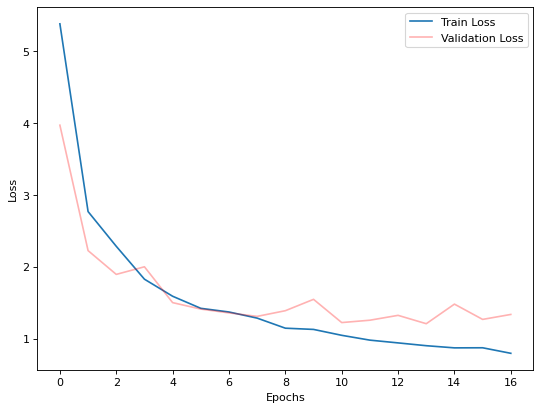
\includegraphics[width=.5\textwidth]{images/training/loss-single-age.png}}
    \caption{Loss trend in the single task for age}
    \label{1loss}
\end{figure}
\begin{figure}[htbp]
    \centerline{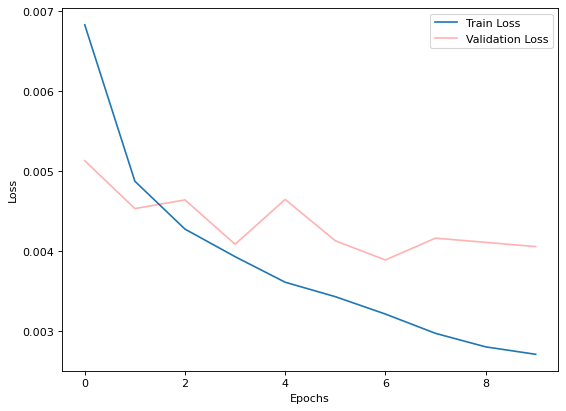
\includegraphics[width=.5\textwidth]{images/training/loss-single-gender.png}}
    \caption{Loss trend in the single task for gender}
    \label{2loss}
\end{figure}
\begin{figure}[htbp]
    \centerline{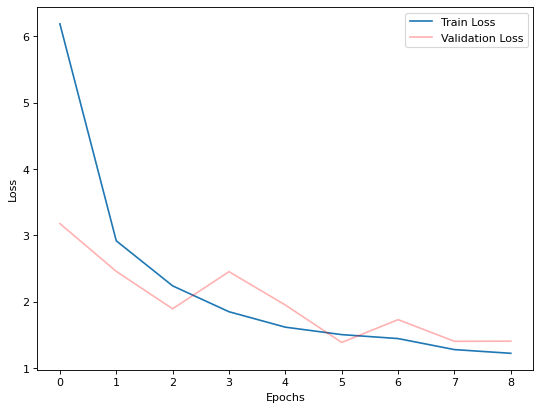
\includegraphics[width=.5\textwidth]{images/training/loss-multi.png}}
    \caption{Loss trend in the multi task}
    \label{3loss}
\end{figure}

\begin{figure}[htbp]
    \centerline{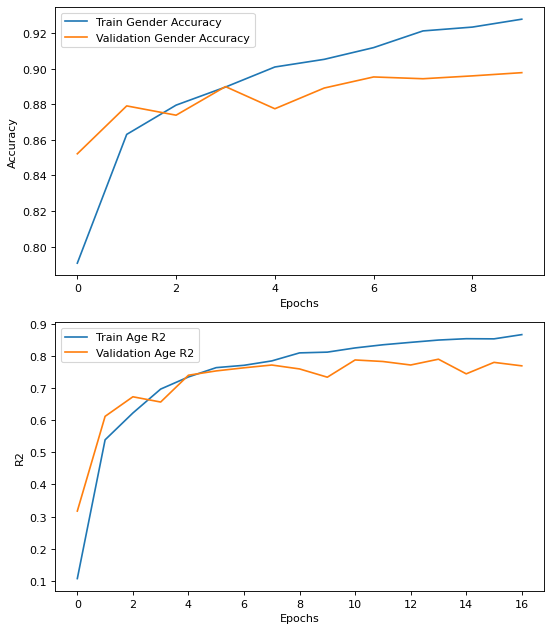
\includegraphics[width=.5\textwidth]{images/training/acc-single.png}}
    \caption{Accuracy trend in the single task CNNs}
    \label{4acc}
\end{figure}
\begin{figure}[htbp]
    \centerline{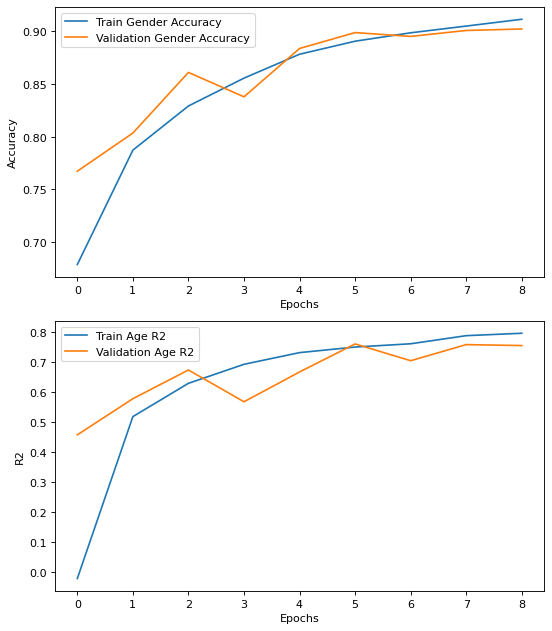
\includegraphics[width=.5\textwidth]{images/training/acc-multi.png}}
    \caption{Accuracy trend in the multi task CNN}
    \label{5acc}
\end{figure}

\subsection{Training Result}

After completing the model training, we can now transition to the testing
phase. During this phase, we load the testing images, which were initially
set aside without undergoing any preprocessing, and evaluate
the capabilities of the CNNs in explaining that data.
Below, you can find the table of accuracy and $R^2$ results for both
architectures:
\begin{table}[H]
    \centering
    \begin{tabular}{@{}lll@{}}
    \toprule
    Metrics & \textbf{Age task ($\mathbf{R^2}$)} & \textbf{Gender task (Accuracy)} \\ \midrule
    \textit{Single-task CNN} &                   &                      \\
    \textit{Multi-task CNN}  &                   &                      \\ \bottomrule
    \end{tabular}
\end{table}
along with Fig.~\ref{6mat} and Fig.~\ref{7mat} illustrating the
confusion matrices for single-task
and multi-task classification, respectively.
\begin{figure}[htbp]
    \centerline{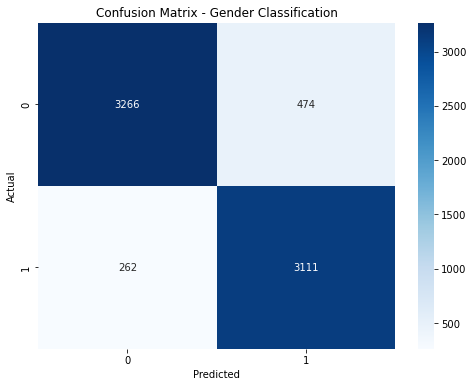
\includegraphics[width=.4\textwidth]{images/testing/mat_single.png}}
    \caption{Confusion Matrix for the single task}
    \label{6mat}
\end{figure}
\begin{figure}[htbp]
    \centerline{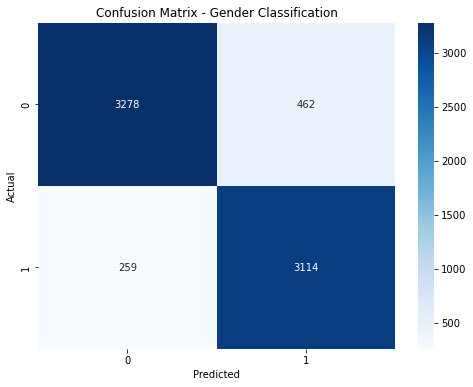
\includegraphics[width=.4\textwidth]{images/testing/mat_multi.png}}
    \caption{Confusion Matrix for the multi task}
    \label{7mat}
\end{figure}
To provide a visual example of the performance of the regressor,
we present, in Fig.~\ref{8reg} and Fig.~\ref{9reg},
a graph depicting the predicted age versus the ground truth
for both the single-task and multi-task scenarios for the first
50 observations of the set.
\begin{figure}[htbp]
    \centerline{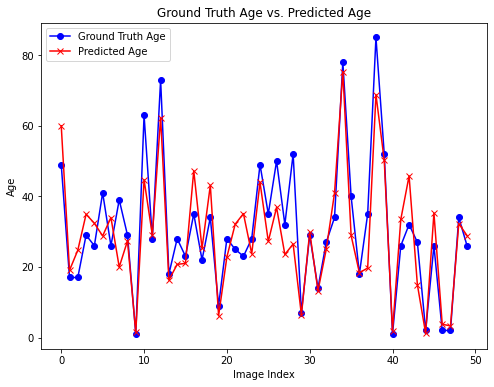
\includegraphics[width=.5\textwidth]{images/testing/reg_single.png}}
    \caption{Regressor performance example for the single task}
    \label{8reg}
\end{figure}
\begin{figure}[htbp]
    \centerline{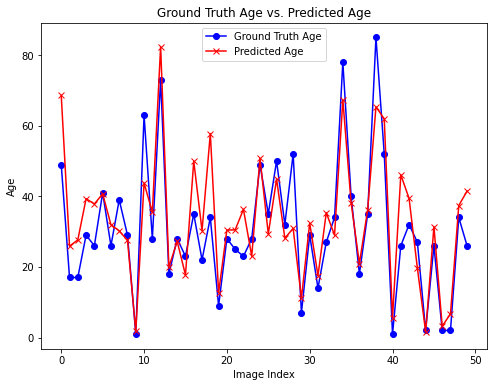
\includegraphics[width=.5\textwidth]{images/testing/reg_multi.png}}
    \caption{Regressor performance example for the multi task}
    \label{9reg}
\end{figure}